\begin{center}\large\textbf{Readings for Correlation and SLR: 10.1-10.5 pg 378-420 and 10.7-10.8 pg 425-444 and 8.7 pg 305-311}\\
\normalsize \end{center}
\large \hlinewd{2pt}
~\\

\textbf{Fit a linear regression model} - A probabilistic model for $Y$ conditional on $X=x$:
		$$ Y_i = \beta_0 + \beta_1 x_i + E_i $$

\textbf{Defintions:}
\begin{itemize}
\item $Y_i$ - response (also called dependent variable)
\item $x_i$ - explanatory variable (also called independent variable or predictor variable)
\item $E_i$ - random error for observation $i$
\item $\beta_0=E(Y|X=0)$ - True population intercept (average value of response when $X=0$
\item $\beta_1$ - True population slope (average change in $Y$ per unit increase in $x$)
\item $\sigma^2$ - Error variance (variance due to experimental error)
\end{itemize}

~\\~\\
Note: We make the assumption that $E_1,\ldots,E_n$ are independent and identically distributed normal random variables with mean 0 and variance $\sigma^2$. We write $E_i \stackrel{iid}{\sim} N(0,\sigma^2)$.  This variance is assumed the same for all $x$, called assumption of \textbf{homoskedasticity}.\\~\\

\begin{center}
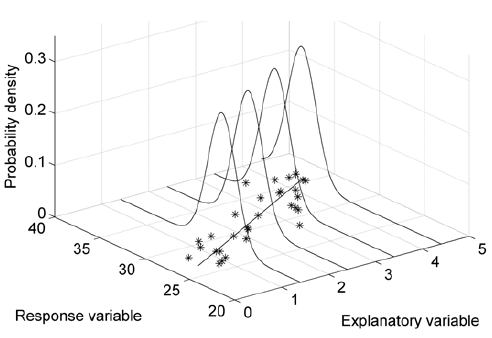
\includegraphics{regnorm}
\end{center}

~\\~\\
\begin{enumerate}
\item $E(Y|X=x)=\beta_0 + \beta_1 x = \mu(x)$ (The line describes the mean $Y$ for a given $X$.)
\item $\Var(Y|X=x)=\sigma^2$
\end{enumerate}

~\\~\\~\\
For the log(Biodiesel) and Biomass example let`s find our fitted line.  Recall the summary stats on page \pageref{bio}.\\
$$\hat\beta_1 = s_{_{XY}}/s_{X}^2 = 3.1485/3.9908^2 =  0.1977$$
$$\hat\beta_0 = 2.4647 - 11.0523*0.1977 = 0.2797$$
$$\hat{y} = 0.2808 + 0.1977x$$

This line can now be used to make predictions for new $X$ values by simply plugging in the $x$!\\

\newpage

Again, we have now have point estimates for our true parameters.  How can we make inference (claims about the true values)?  Do we have a \textit{significant linear relationship}?\\
Under the normal distribution assumption on the errors, the RV`s $\hat\beta_0$ and $\hat\beta_1$ follow normal distributions.  Thus, we can use this as a basis for inference.\\~\\

What value of the slope do we test?
\begin{itemize}
\item If a linear relationship, $Y$ will tend to change with $X$ (i.e. $\beta_1 \ne 0$)
\item If no linear relationship, $Y$ won`t tend to change with $X$ (i.e. $\beta_1 = 0$).
\end{itemize}

\begin{center}
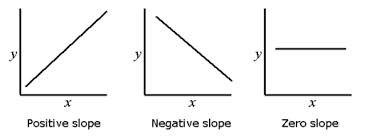
\includegraphics{SLR1}
\end{center}

~\\~\\
Any hypothetical slope, like \fbox{$H_0:\beta_1=\mbox{slope}_0$} may be tested using the $T$-statistic below with $df=n-2$:
$$ T=\frac{\hat\beta_1-\mbox{slope}_0}{\widehat{SE}(\hat\beta_1)}$$ 
and any hypothetical intercept, like \fbox{$H_0:\beta_0=\mbox{intercept}_0$} may be tested using the $T$-statistic below with $df=n-2$:
$$ T=\frac{\hat\beta_0-\mbox{intercept}_0}{\widehat{SE}(\hat\beta_0)}$$ 

\cu{Confidence intervals for $\beta_0, \beta_1$}
$100(1-\alpha)\%$ confidence intervals for $\beta_0$ and $\beta_1$ are 
given by 
$$\hat{\beta}_0 \pm t(n-2,\alpha/2) \sqrt{MS[E]\left(\frac{1}{n}+\frac{\bar{x}^2}{S_{xx}}\right)}. $$
$$\hat{\beta}_1 \pm t(n-2,\alpha/2) \sqrt{\frac{MS[E]}{S_{xx}}}. $$

Often we will only care about the test and CI for the slope.  The hypothesis test is equivalent to checking if 0 is in the confidence interval.  It will depend on the context of the question if testing $\beta_0$=0 makes sense.\\~\\

\textbf{Confidence interval for $\mu(x_0) = E(Y|X=x_0)$}\\
The point estimate for $\mu(x_0)$ is simply $\hat\beta_0+\hat\beta_1x_0$.  We need to know about the variability of this estimate and we can again use the t-distribution for inference.

\begin{eqnarray*}
\Var(\hat\beta_0+\hat\beta_1 x_0|X=x_0)
& = & 
\end{eqnarray*}
This yields a confidence interval of the form
$$\hat\beta_0 +\hat\beta_1 x_0 \pm t(n-2,\alpha/2) \sqrt{MS[E]\left(\frac{1}{n}+\frac{(x_0-\bar{x})^2}{S_{xx}}\right)} $$
Note: We are attempting to capture the true \textit{mean} at $x_0$ in this interval.\\~\\

\textbf{Prediction interval for a new observation $x_0$}\\
The point estimate for at $x_0$ is still $\hat{Y}(x_0)=\hat\beta_0+\hat\beta_1x_0$.  However, the variability will change.
\begin{eqnarray*}
\Var(\hat\beta_0+\hat\beta_1 x_0+E_{new}|X=x_0)
& = & 
\end{eqnarray*}

Thus we can form a PI using
$$ \hat{Y}(x_0) \pm t(n-2,\alpha/2) \sqrt{MS[E]\left(1+\frac{1}{n}+\frac{(x_0-\bar{x})^2}{S_{xx}}\right)}. $$
Note: In this interval we are attempting to capture the next $Y$ value that takes on $x_0$.  As this is a much more difficult task, PI`s are wider than CI`s.  \\~\\

\newpage

\cu{The ANOVA table from simple linear regression}

The full ANOVA table for SLR is given below:\\
\begin{tabular}{|c|c|c|c|c|} \hline
Source & Sum of squares & df & Mean Square & F-Ratio \\ \hline
Regression & $SS(R)$ & 1 & $MS(R)$ & $MS(R)/MS(E)$ \\
Error & $SS(E)$ & $n-2$ & $MS(E)$ &  \\
Total & $SS(Tot)$ & $n-1$ & &  \\ \hline
\end{tabular}

~\\
The mean squares represent standardized measures of variation due to the different sources and are given by $SS(source)/df source$.  Ratios of mean squares often follow an $F$-distribution and are appropriate for testing different hypotheses of interest.\\~\\
In this case, to test 
$$ H_0: \beta_1 = 0 \ \ \ \ \mbox{ vs }\ \ \ \ H_1:\beta_1 \neq 0$$
$F = MS(R)/MS(E) \sim F(1,n-2)$.\\~\\
That is, the $F$ statistic follows an $F$-distribution with 1 numerator df and $n-2$ denominator df.  In SLR, this $F$ test is equivalent to the $T$ test we already looked at.  The relationship is that $T^2=F$.  \\~\\
Note:  The mean square for error, $MS[E]$, is an unbiased estimator for $\sigma^2$.  It is an estimate of the variability due left over once we account for our explanatory variable.  

\newpage

\textbf{How to get tests in SAS?}\\
For our Biodiesel and Biomass example we can get much of our output from SAS using the following commands:\\
\begin{small}
\begin{verbatim}
proc reg data=bioexp ;
model logbiodiesel=biomass/clb;
run;
\end{verbatim}
\end{small}
~\\
\begin{center}
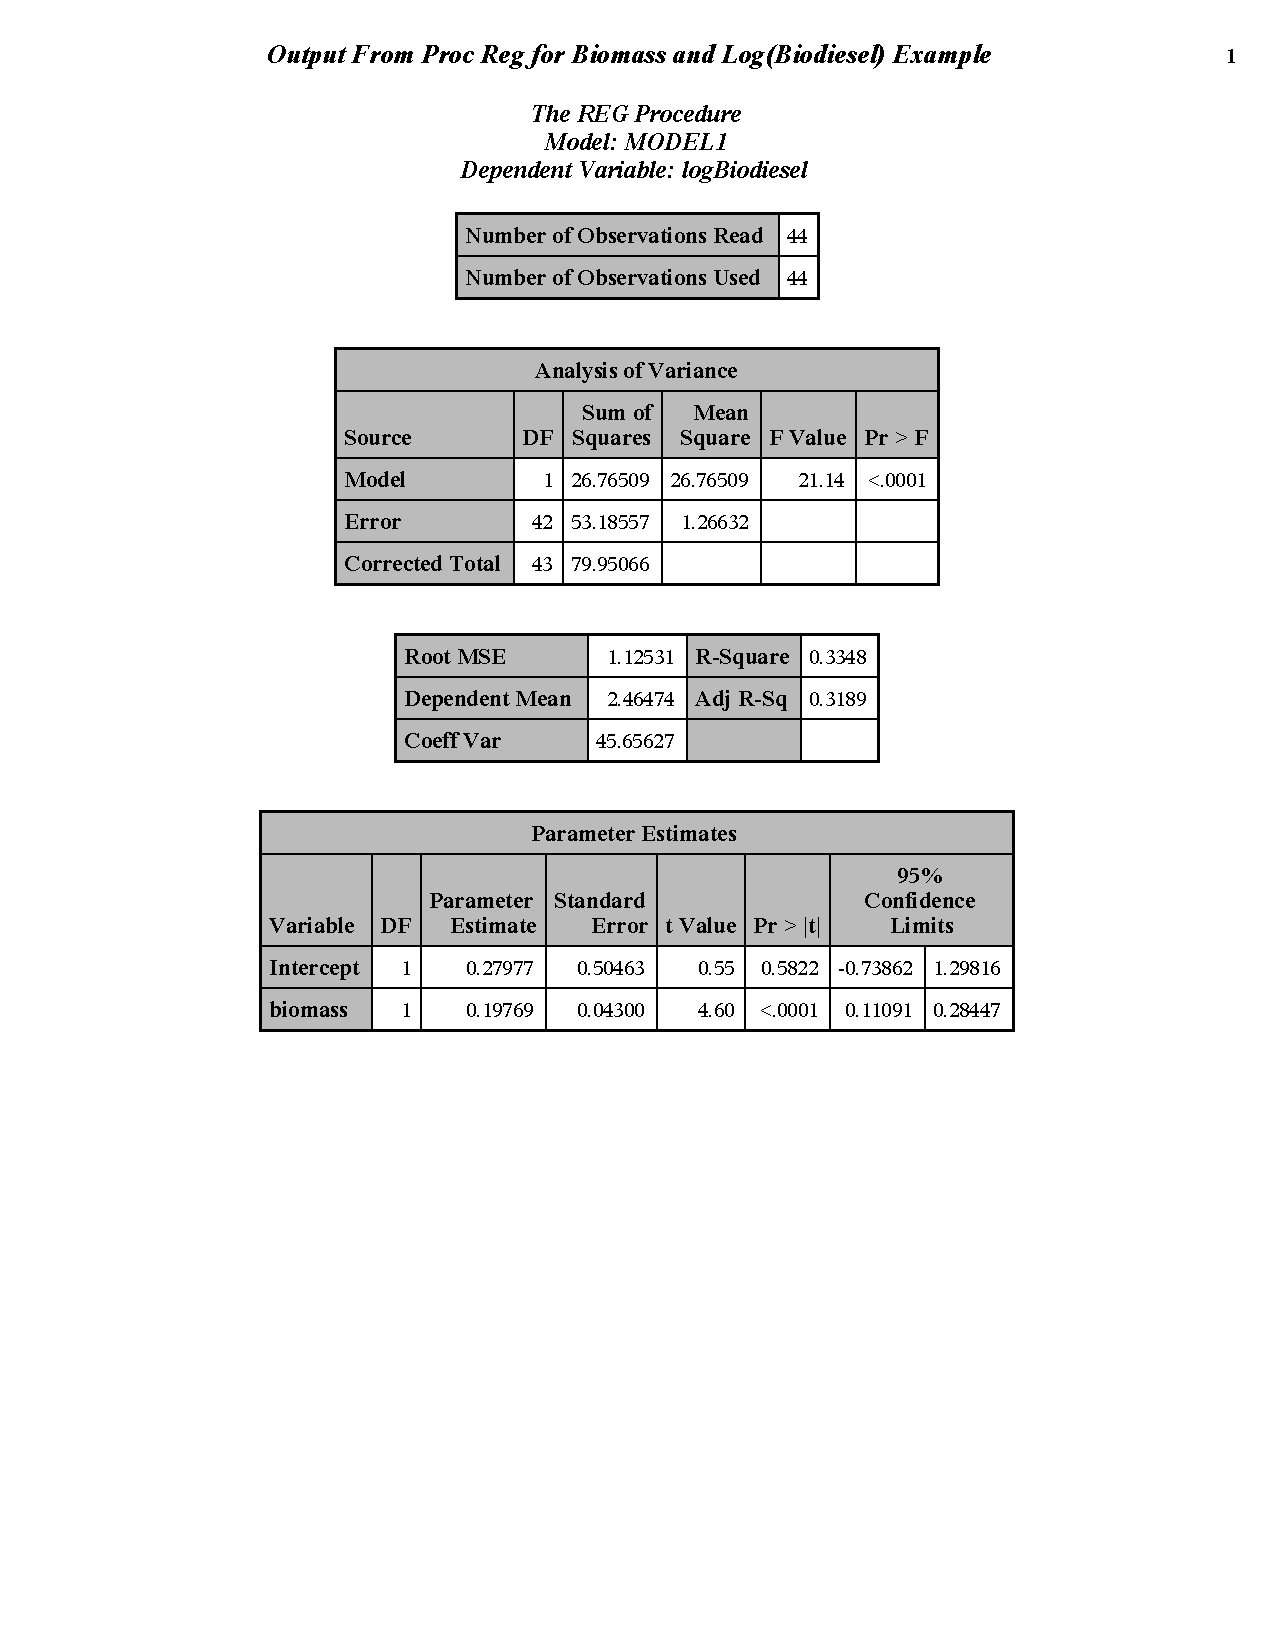
\includegraphics[scale=0.7,trim= 10mm 105mm 10mm 10mm]{slrbiodiesel}\\
\end{center}

~\\~\\
Using $\alpha=0.05$, (1) let`s find the CI for the slope by hand, (2) form a CI for the mean log of biodiesel when biomass is 12, and (3) form a PI for a future log biodiesel measurement for a biomass of 12.\\

\newpage


SAS will also produce a very nice plot that includes \textit{pointwise} confidence and prediction bands at all points. Notice that the bands get wider the further $x_0$ is from $\bar{x}$.  Why?

\begin{center}
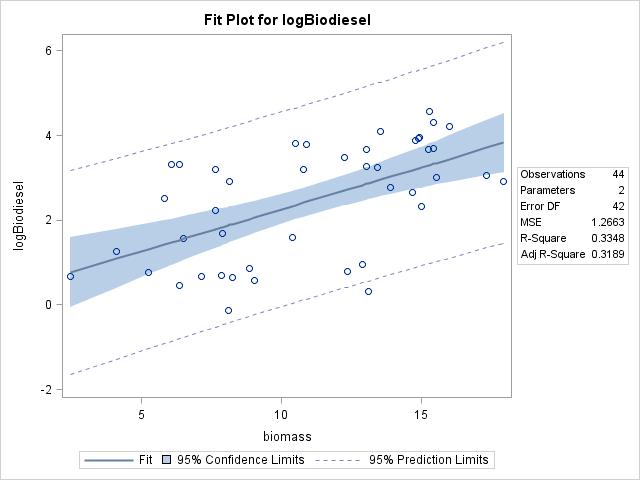
\includegraphics[scale=0.55]{biofitpred}
\end{center}

~\\~\\~\\
\textbf{Checking assumptions}\\
Firstly, we should always inspect a scatter plot to determine if the linear relationship we are assuming in our model is appropriate.\\~\\
Secondly we can check our assumption of $iid N(0,\sigma^2)$ errors.  
\begin{itemize}
\item Independence - There is not a check for independence of errors,  we simply need to consider whether or not our EUs can be considered independent. 
\item Constant variance - A residuals vs fitted (predicted) values plot or a residual vs independent variable plot are tools for detecting heteroskedasticity (non-constant variance).  
\begin{center}
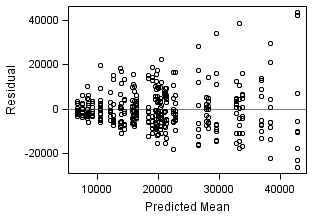
\includegraphics{hetero}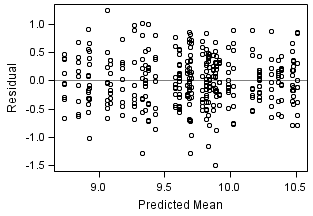
\includegraphics{homo}
\end{center}
\item Normality of errors - A quantile-quantile plot (or qq-plot for short) can be inspected to see if normality is reasonable.
\begin{center}
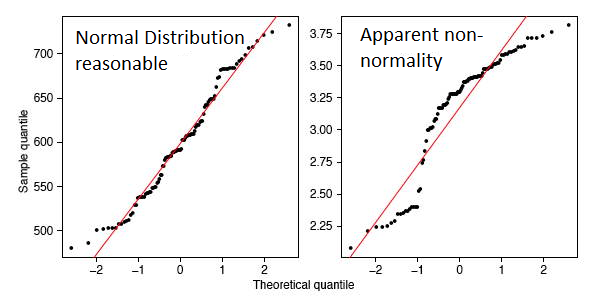
\includegraphics[scale=0.5]{qq}
\end{center}
\end{itemize}

We can inspect the diagnostic plots that SAS produces when the reg procedure is used:
\begin{center}
\includegraphics[scale=0.7,page=2,trim= 10mm 70mm 10mm 10mm]{slrbiodiesel}\\
\includegraphics[scale=0.4,page=3,trim= 10mm 100mm 10mm 10mm]{slrbiodiesel}
\end{center}

\textbf{An exercise: Match up letters a,b,c,d with the model violation - Heteroscedasticity, Nonlinearity, Nonnormality, Model fits}
\begin{center}
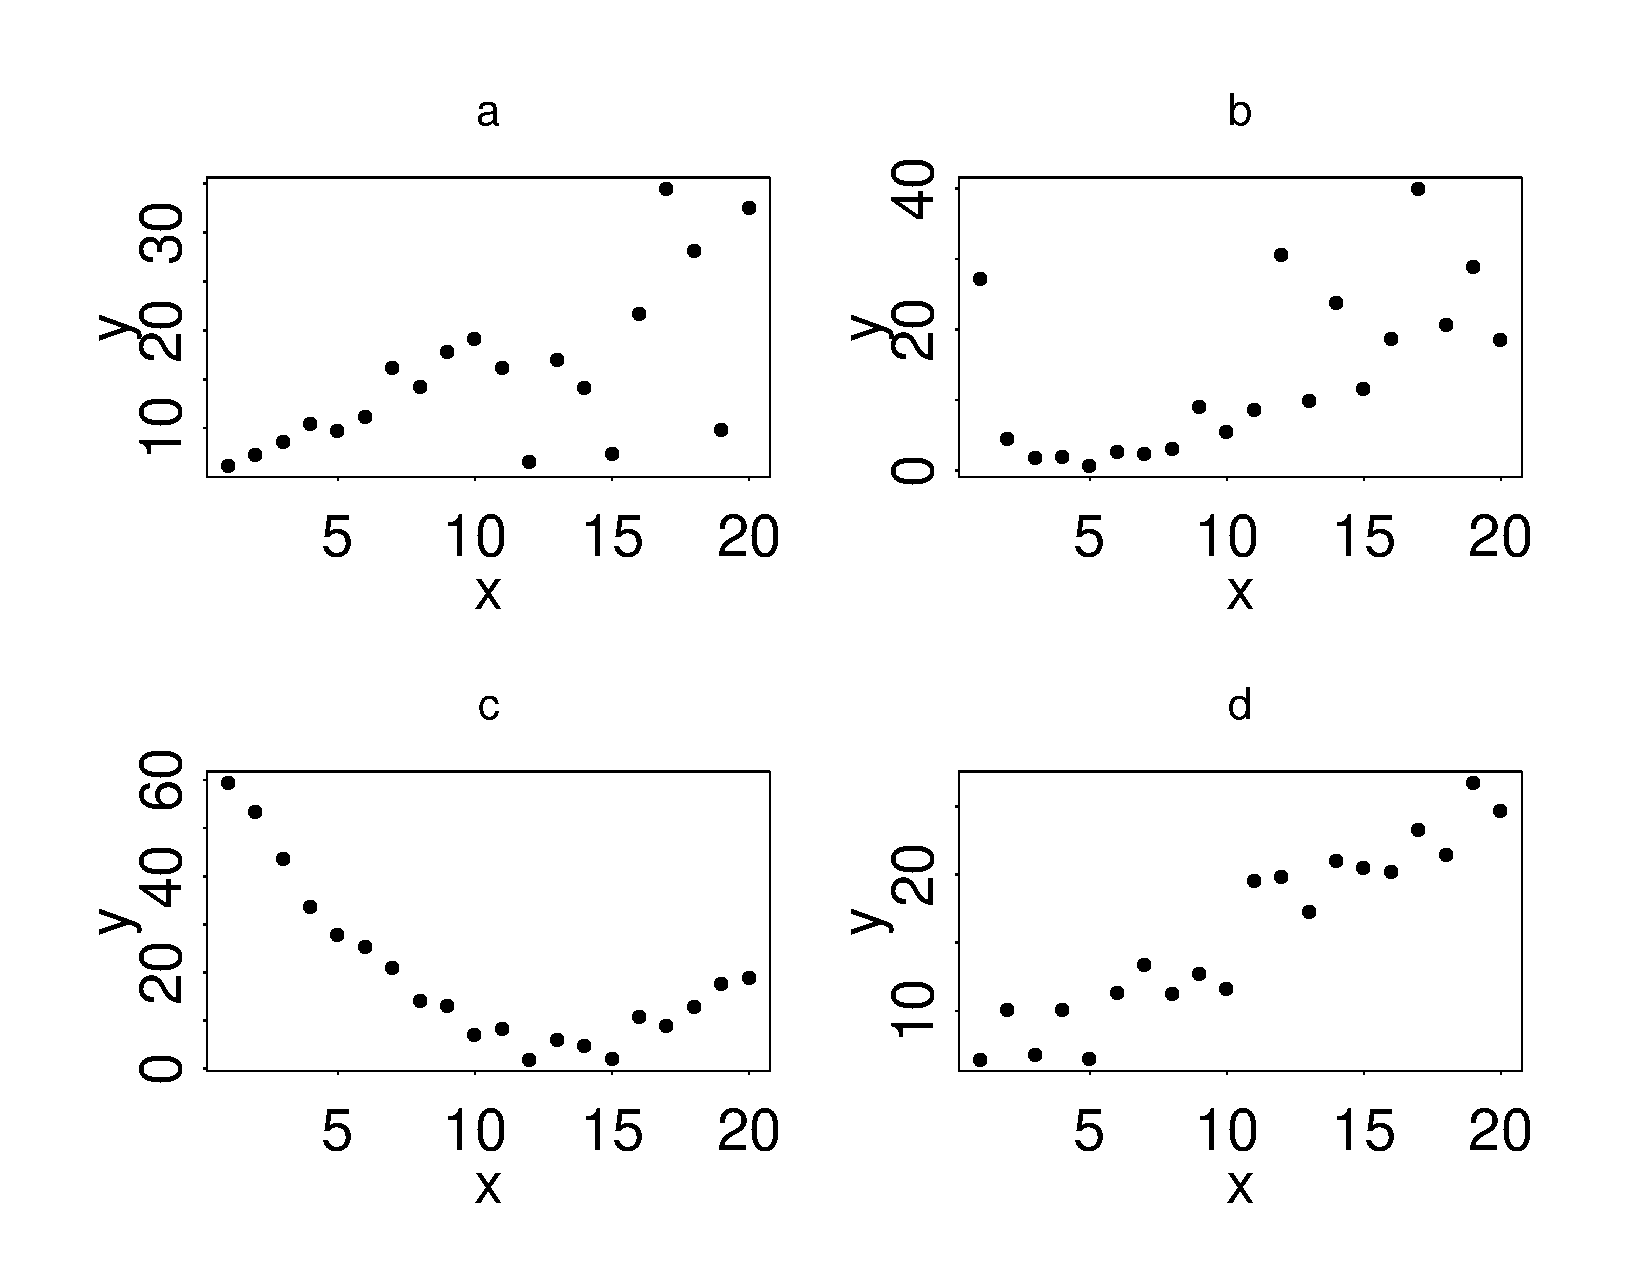
\includegraphics[height=2.5in,width=3in]{ybyx_handout.pdf}
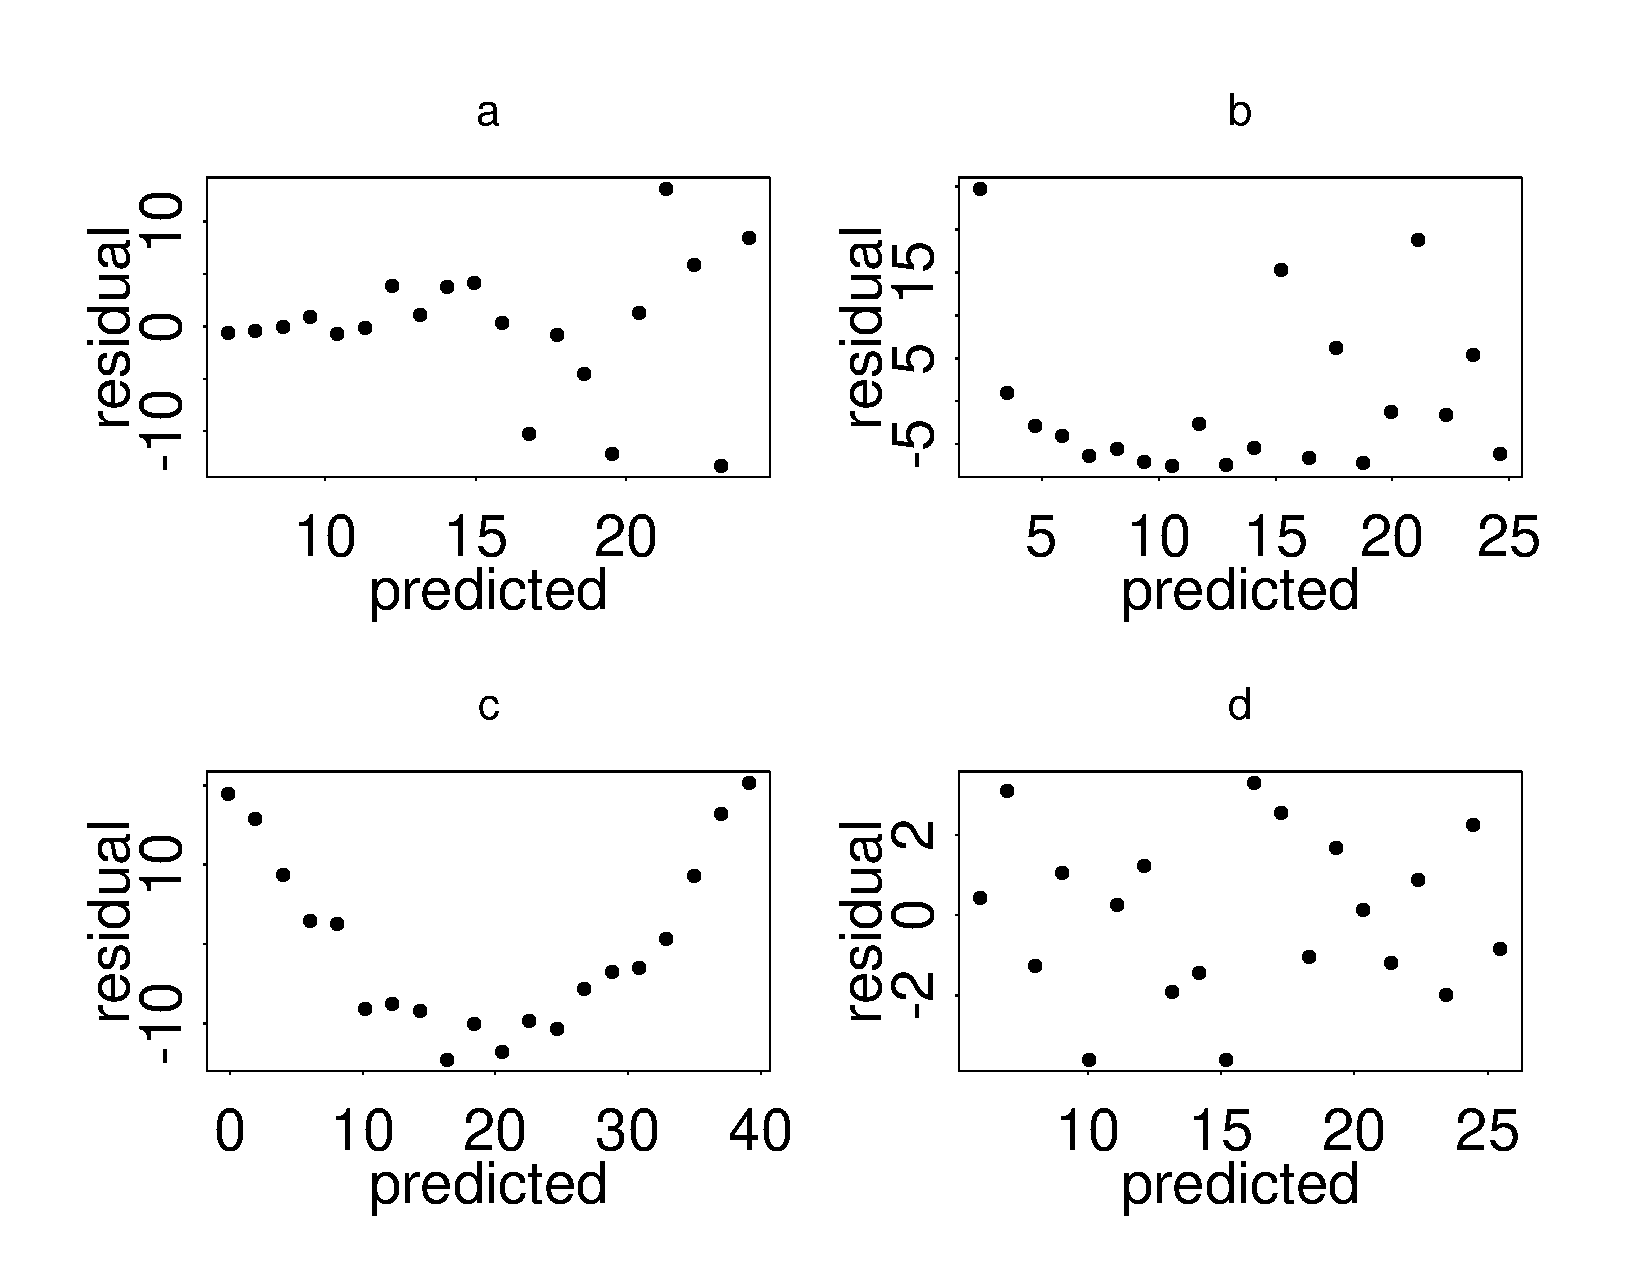
\includegraphics[height=2.5in,width=3in]{resbypred_handout.pdf}
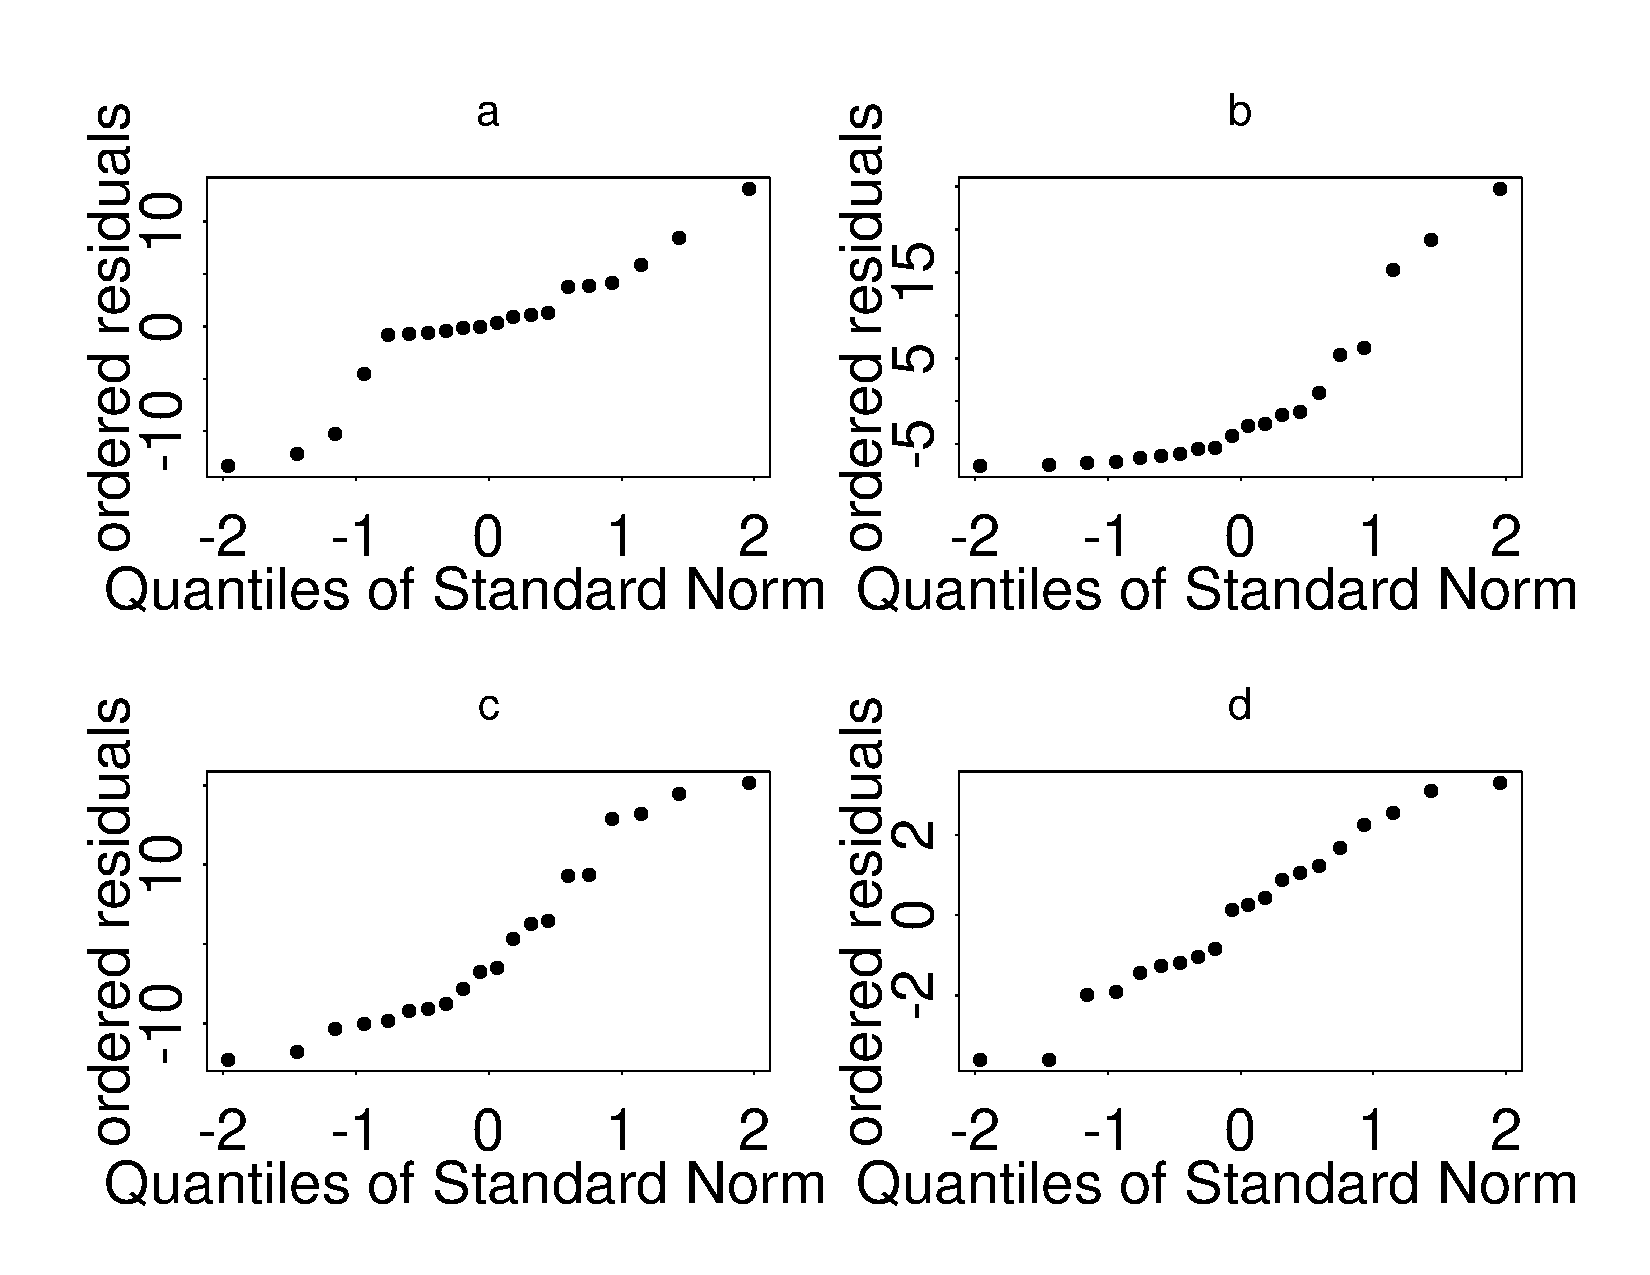
\includegraphics[height=2.5in,width=3in]{qqnorm_handout.pdf}
\end{center}



